\documentclass{article}

\usepackage[preprint]{neurips_2025}

\usepackage[utf8]{inputenc}
\usepackage[T1]{fontenc}
\usepackage{hyperref}
\usepackage{url}
\usepackage{booktabs}
\usepackage{amsfonts}
\usepackage{amsmath}
\usepackage{nicefrac}
\usepackage{microtype}
\usepackage{xcolor}
\usepackage{graphicx}

\title{Assignment 3: Conditional Jet Generation with Flow Matching}

\author{%
  Leonardo Mattos Martins \\
  Boston University
}

\begin{document}

\maketitle

\begin{abstract}
We train a conditional flow-matching model for JetNet particle clouds conditioned on jet type (g, q, t, W, z). Relative to the starter baseline, we use a masked set-aware architecture with time/type conditioning, mask-weighted training, and EMA parameters, and we sample with RK2 (Heun) integration. On the validation set, the final composite Wasserstein-1 score is \textbf{0.03820} (lower is better). Qualitative plots show that generated jets reproduce the main observable distributions and recover realistic prong-like structure in the $\eta$-$\phi$ plane.
\end{abstract}

\section{Approach}

I frame the task as conditional flow matching (CFM) on masked particle clouds with up to 30 particles per jet. I started from the provided flat MLP baseline and then iterated on architecture, features, optimization, and sampling, with the goal of improving the composite W1 metric while preserving physically realistic jet structure.

\textbf{What I tried and why:}
\begin{itemize}
    \item \textbf{Set-aware architecture instead of flattening.} Flattening loses permutation structure and weakens particle--particle interaction modeling. I therefore used a masked self-attention velocity network with residual feed-forward blocks and masked global pooling so the model can capture multi-prong substructure.
    \item \textbf{Stronger conditioning.} I used sinusoidal time embeddings and learned jet-type embeddings, injected through FiLM-style modulation. This gives the network direct control over trajectory dynamics across diffusion time and class.
    \item \textbf{Feature and mask handling.} The model predicts per-particle velocities $(\dot{\eta}_{rel},\dot{\phi}_{rel},\dot{p}_T^{rel})$ and enforces zero output on padded slots. This keeps training and generation consistent with variable-length jets.
    \item \textbf{Training stabilizers.} I used a mask-aware CFM objective with interpolation $x_t=(1-t)x_0+t x_1$, a U-shaped Beta-biased time schedule, gradient clipping, AdamW with warmup/cosine decay, and EMA parameters. These were chosen to improve stability and sample quality on large-batch TPU training.
    \item \textbf{Higher-quality integration.} I replaced Euler sampling with RK2 (Heun) to reduce discretization error at fixed step count, since sampling error directly affects final W1.
\end{itemize}

I also ran a controlled model comparison (flat MLP, DeepSets, EGANN, and attention-based model) under the same training/evaluation protocol. This helped isolate which inductive biases mattered most and motivated selecting the attention-based masked set model as the final submission model.

\section{Results and Analysis}

Table~\ref{tab:w1} reports the validation W1 breakdown for the final model. The composite score is \textbf{0.03820}. The best per-type totals are for gluon, top, and $Z$ jets, while quark jets are the hardest among the five types in this run.

Across observables, mass and $p_T^{rel}$ dominate the error budget more than angular coordinates. This matches the qualitative behavior in Figure~\ref{fig:observables}: generated distributions closely match real data in central regions, while heavier tails and sharper structures are still slightly smoothed.

The $\eta$-$\phi$ examples in Figure~\ref{fig:etaphi} show that generated jets capture realistic spatial concentration and multi-prong tendencies, especially for top/W/Z classes. Remaining failure modes are occasional over-diffusion and less distinct prong separation in difficult jets, which likely reflects finite model capacity and integration discretization.

\begin{table}[t]
\centering
\caption{Validation W1 scores ($\downarrow$) for the final model by jet type and observable.}
\label{tab:w1}
\begin{tabular}{@{}lccccc@{}}
\toprule
Observable & Gluon & Quark & Top & $W$ & $Z$ \\
\midrule
Mass & 0.00092 & 0.00604 & 0.00175 & 0.00368 & 0.00364 \\
$\eta_{rel}$ & 0.00136 & 0.00152 & 0.00115 & 0.00119 & 0.00050 \\
$\phi_{rel}$ & 0.00162 & 0.00181 & 0.00147 & 0.00075 & 0.00046 \\
$p_T^{rel}$ & 0.00231 & 0.00231 & 0.00205 & 0.00177 & 0.00189 \\
\midrule
Per-type total & 0.00621 & 0.01169 & 0.00641 & 0.00739 & 0.00649 \\
\bottomrule
\end{tabular}
\\[0.3em]
\small Composite total across all jet types and observables: \textbf{0.03820}.
\end{table}

\begin{figure}[t]
    \centering
    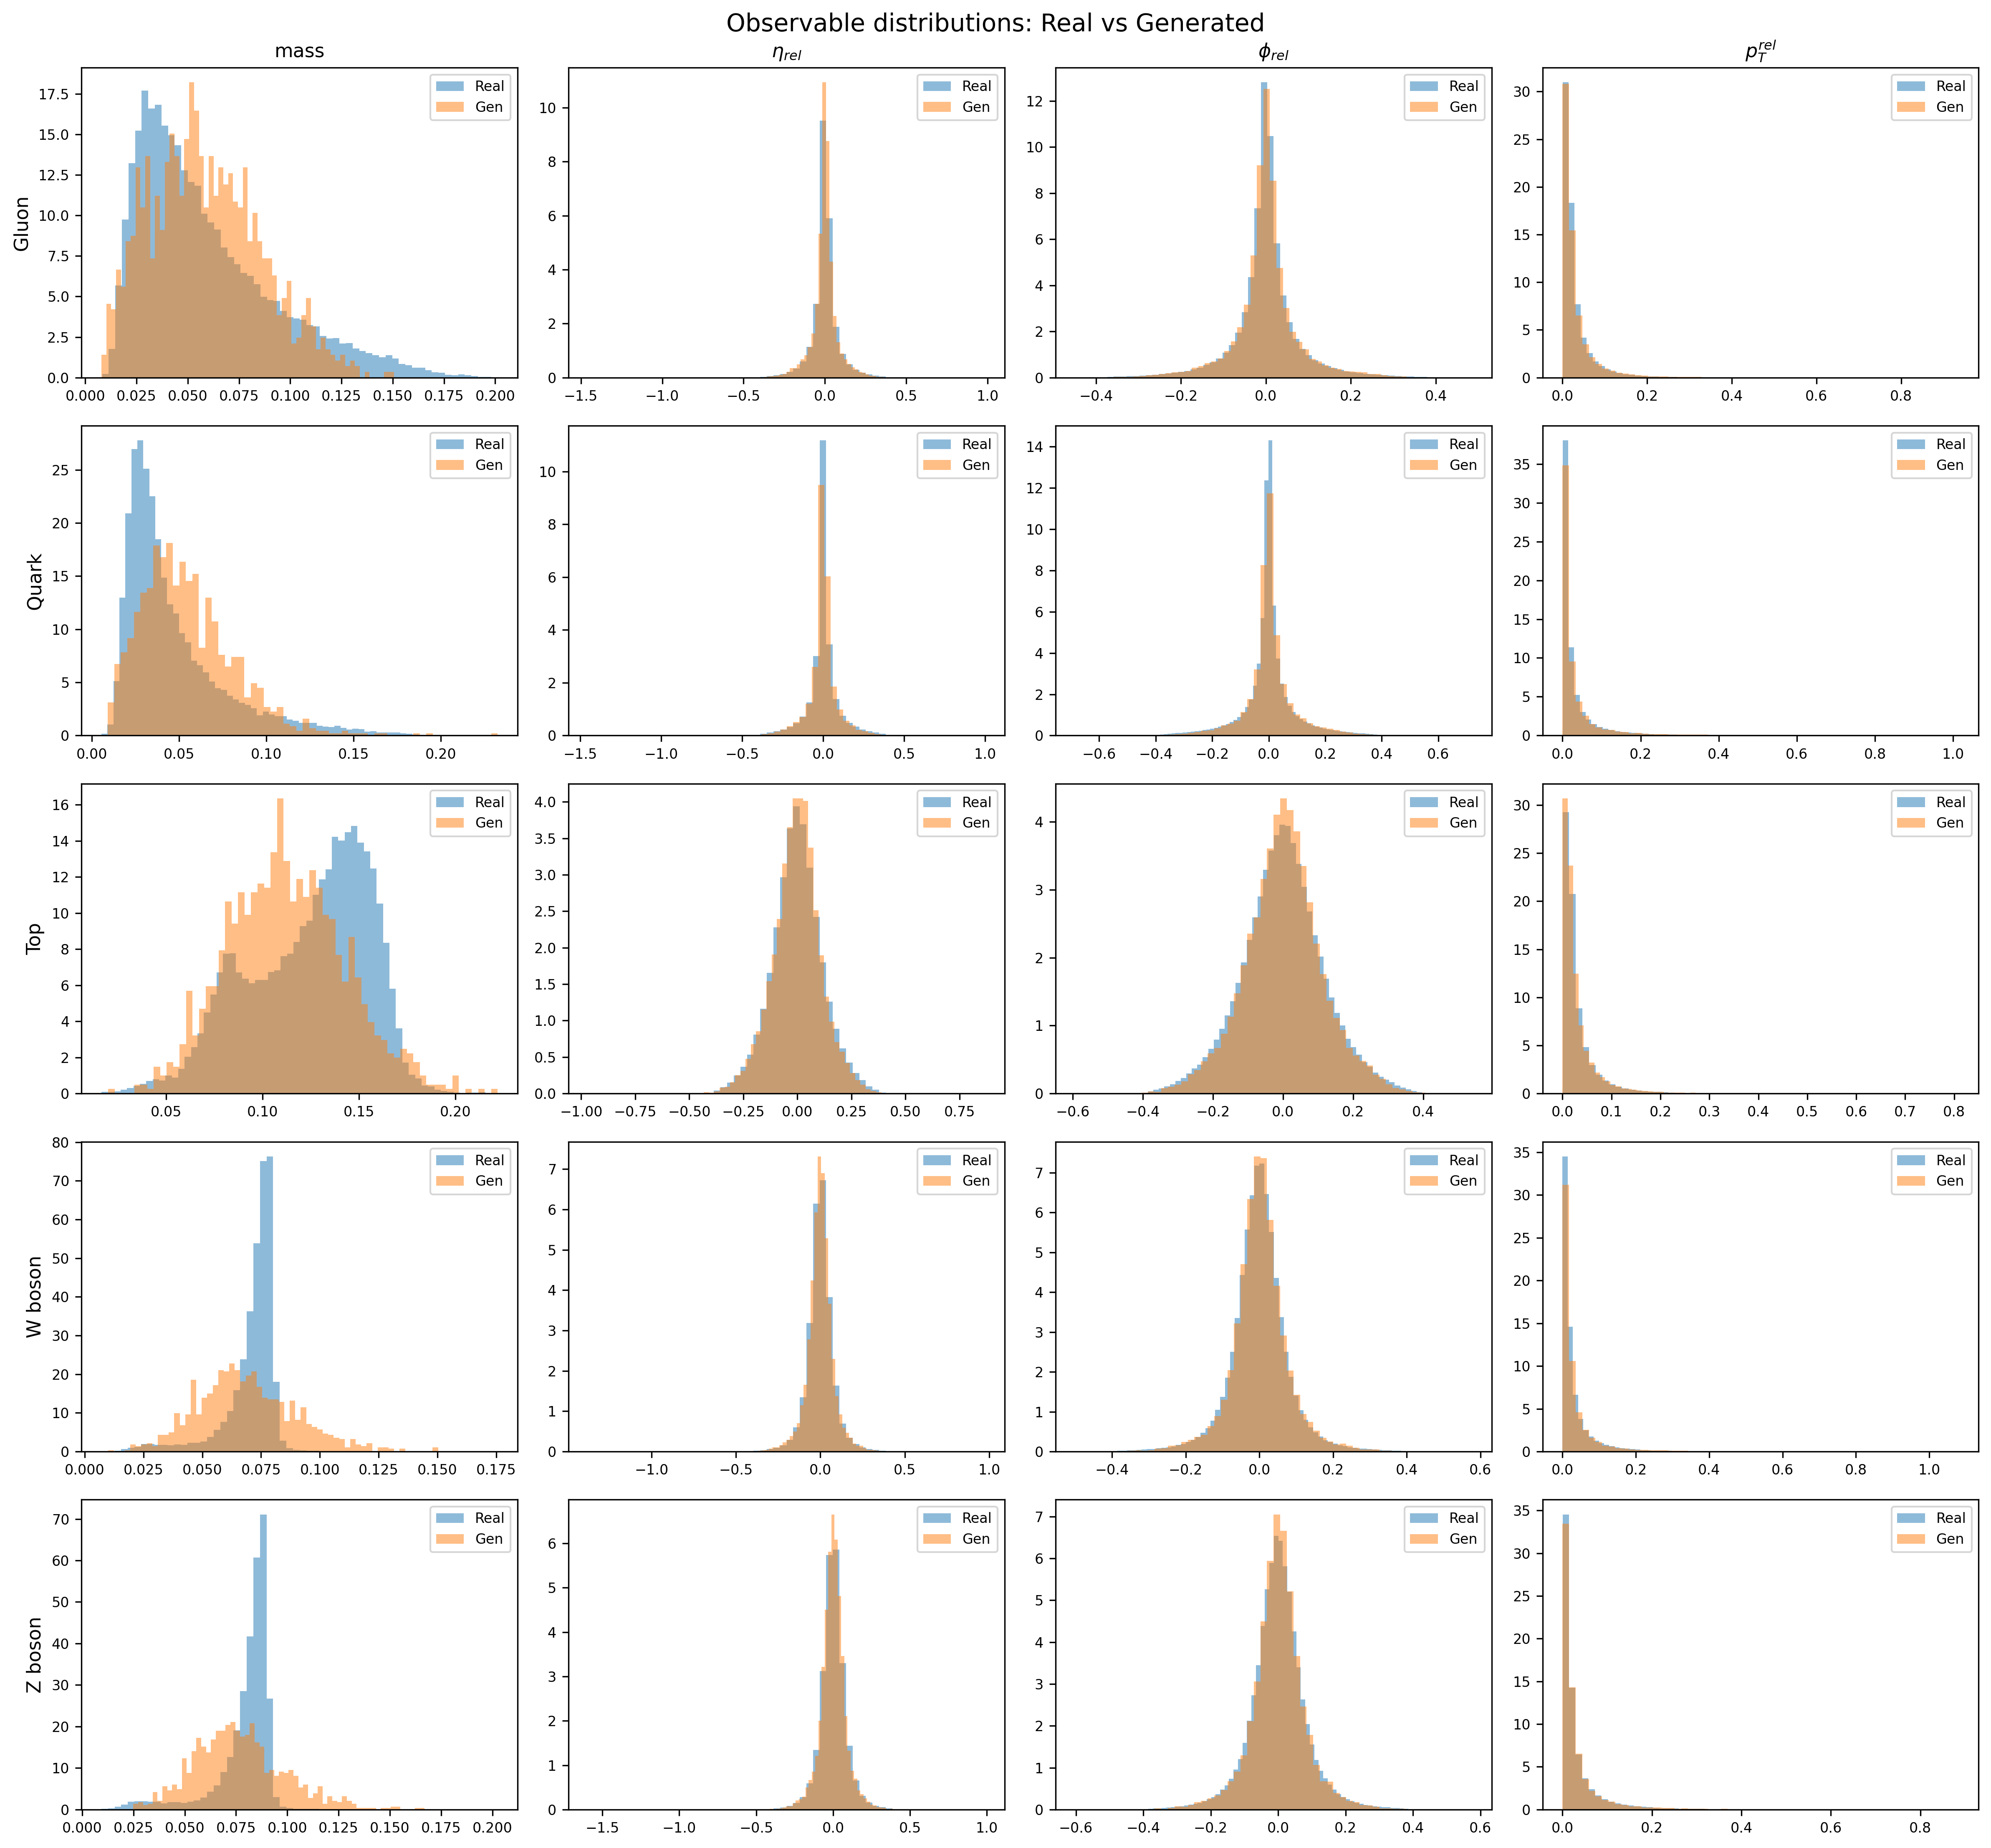
\includegraphics[width=\linewidth]{figures/observables_real_vs_generated.png}
    \caption{Observable distributions for real vs generated jets (mass, $\eta_{rel}$, $\phi_{rel}$, $p_T^{rel}$) across all five jet types.}
    \label{fig:observables}
\end{figure}

\begin{figure}[t]
    \centering
    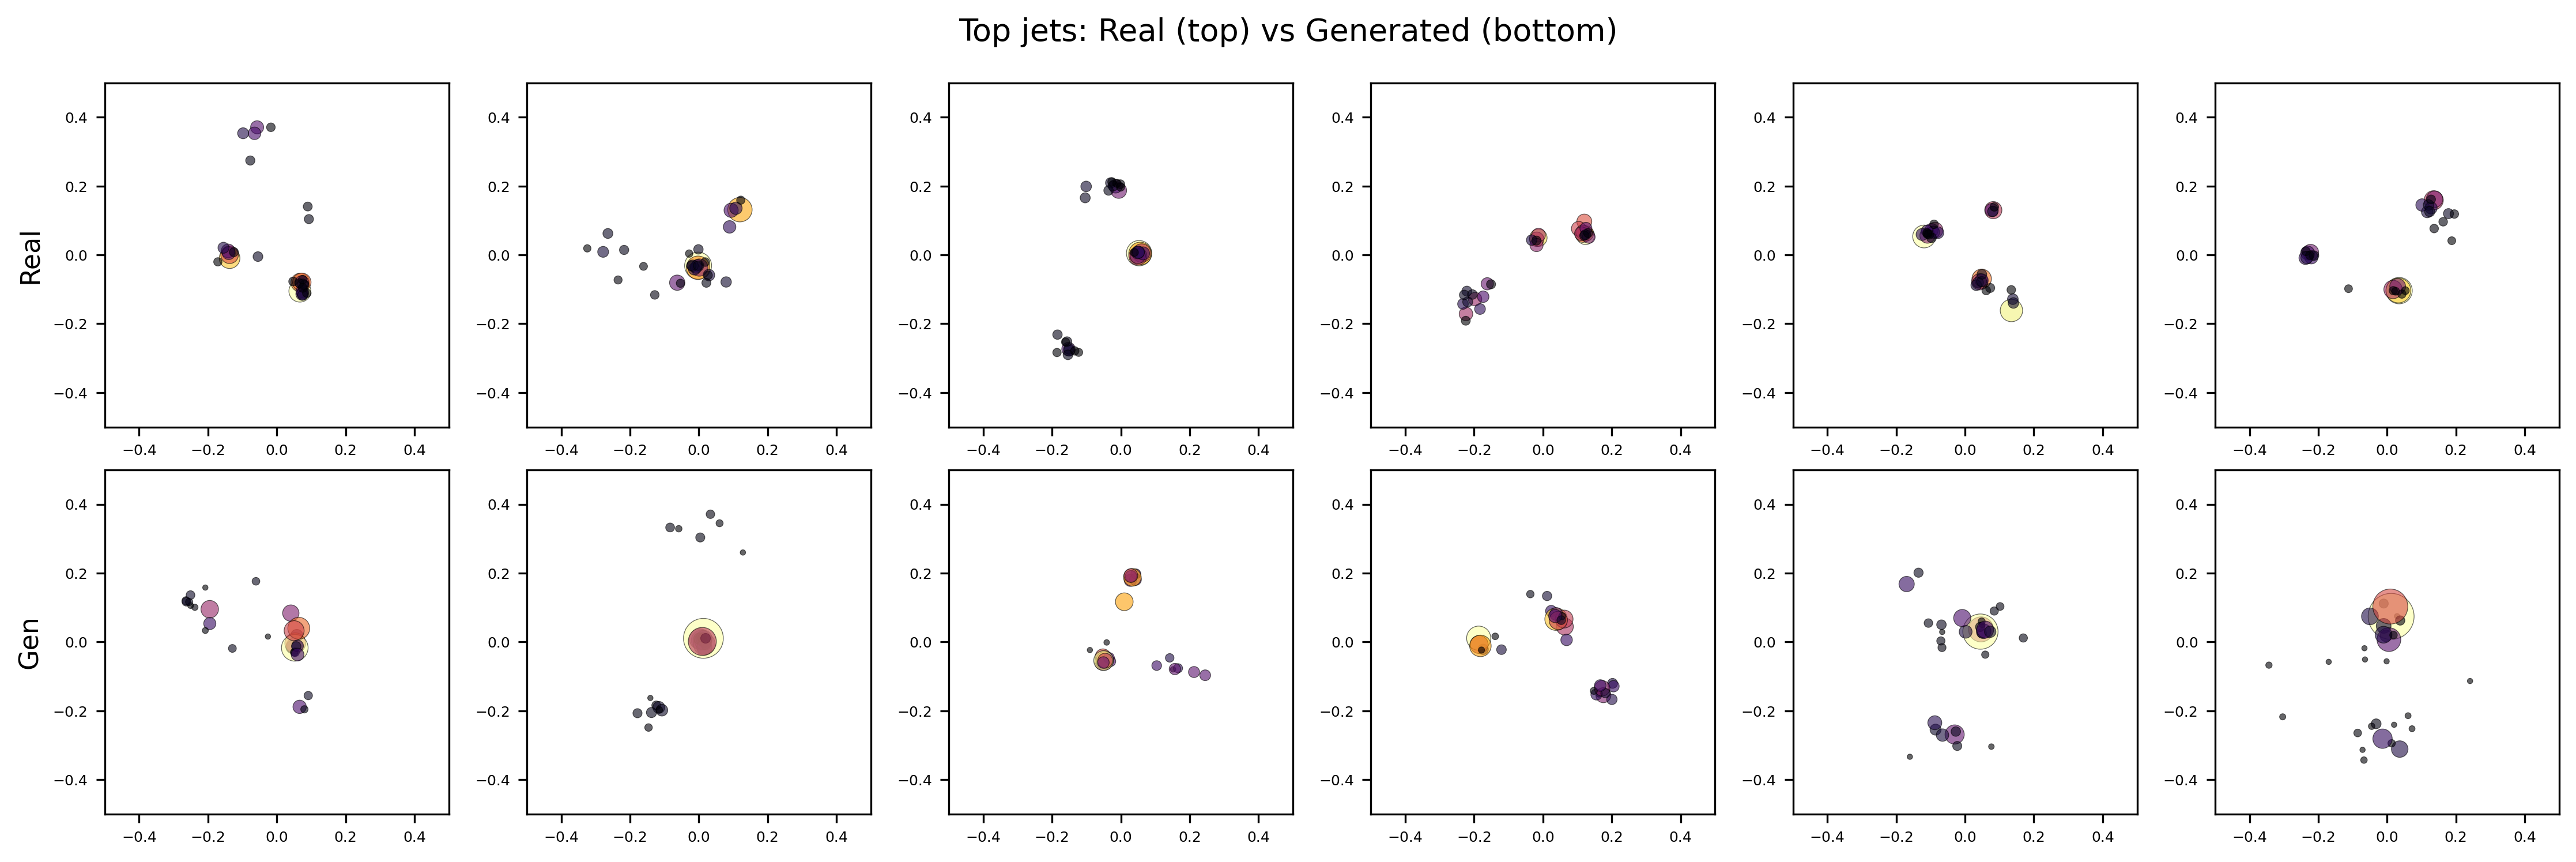
\includegraphics[width=0.49\linewidth]{figures/eta_phi_real_vs_generated_t.png}
    \hfill
    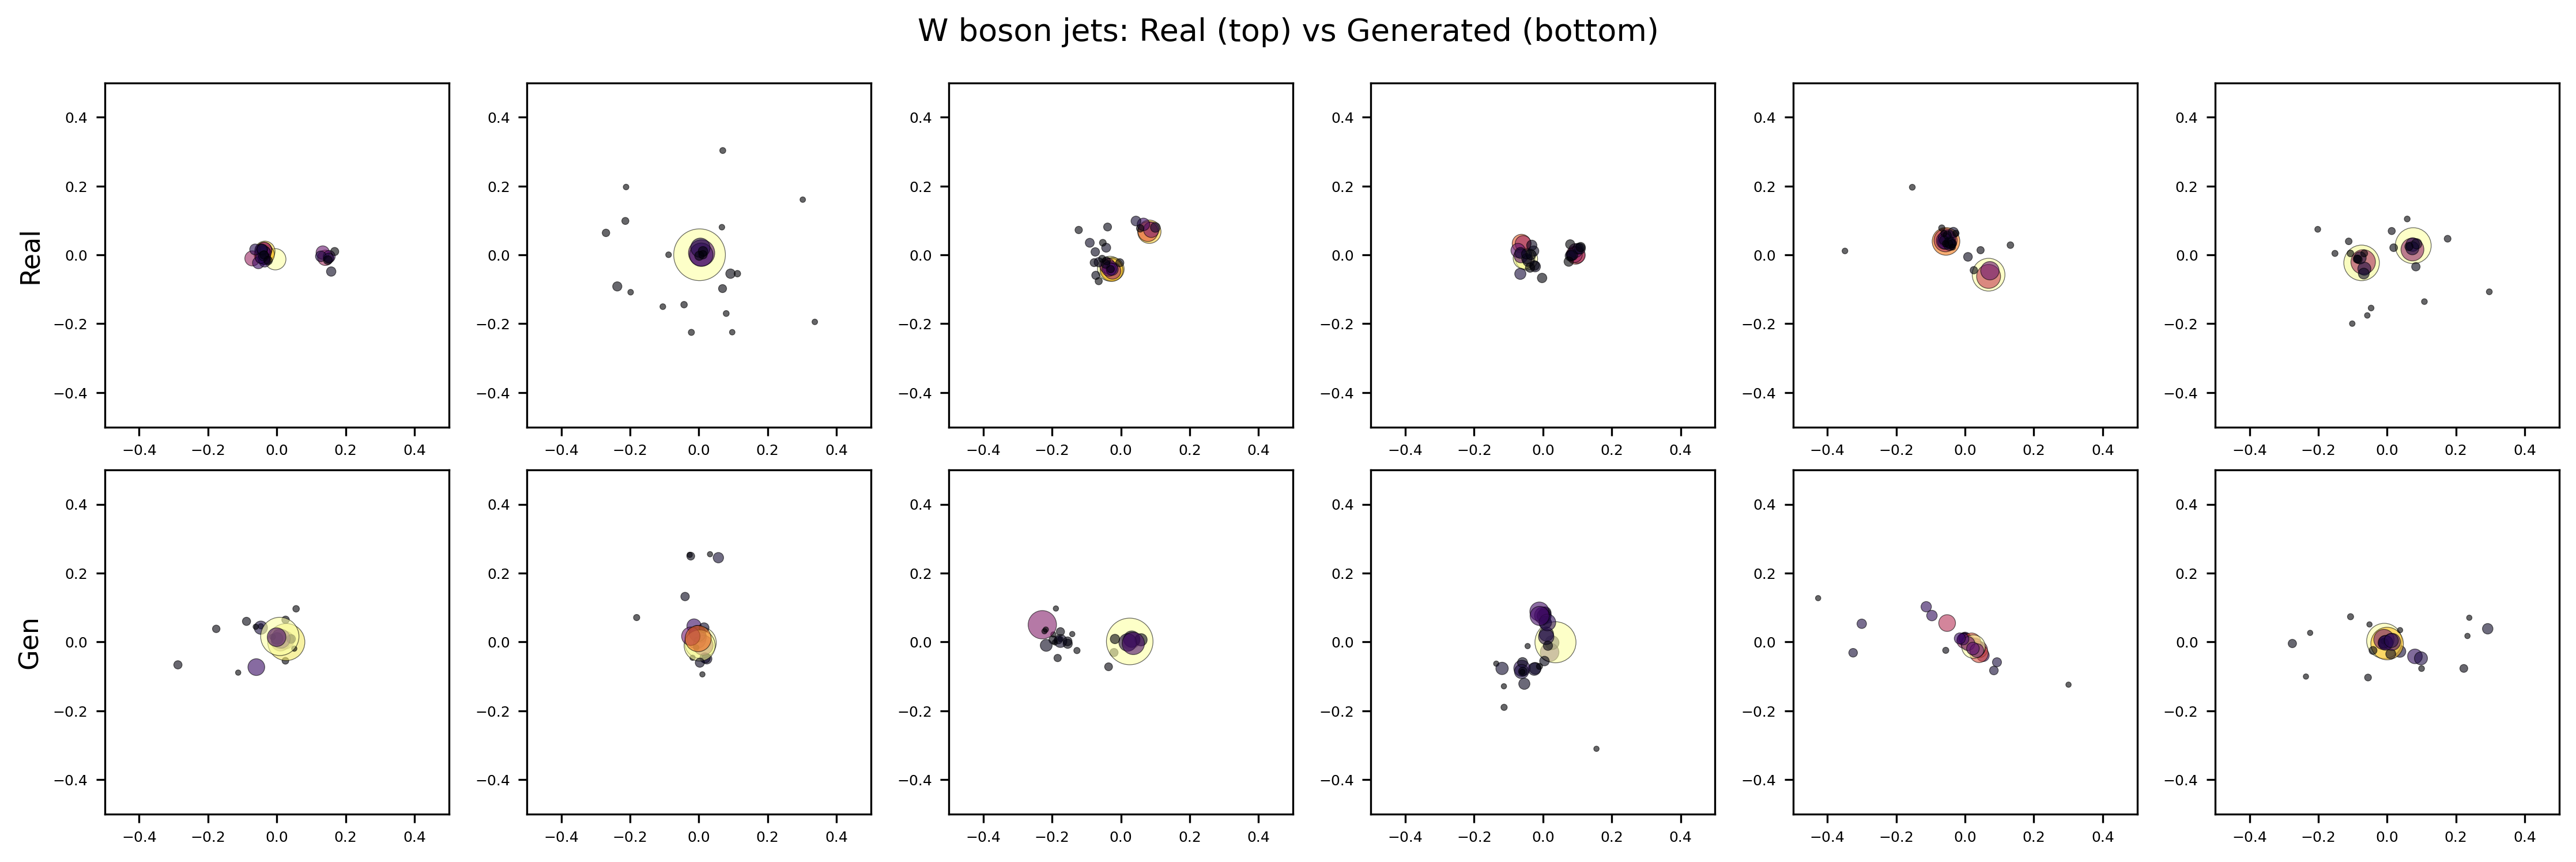
\includegraphics[width=0.49\linewidth]{figures/eta_phi_real_vs_generated_w.png}
    \caption{$\eta$-$\phi$ real-vs-generated comparisons for representative heavy-object classes (top and $W$).}
    \label{fig:etaphi}
\end{figure}

\section{AI Collaboration}
I used Gemini and the Windsurf IDE to develop this project. During ideation, I prompted Gemini to ruthlessly critique my strategy. The model provided ratings and explanations which I used to fix flaws and improve the design. This approach was effective because it forced me to find errors that I had missed.

For implementation, I used Windsurf to manage file sharing. The tool synced my local repository with the virtual file system for the Google Colab plugin. My analysis shows that using Gemini as a critic instead of a writer was the best strategy. It removed bias from the planning stage. Windsurf also reduced the work needed to move code between my computer and the cloud. This combination made the final strategy stronger and the technical setup more reliable.

\end{document}
